% Options for packages loaded elsewhere
\PassOptionsToPackage{unicode}{hyperref}
\PassOptionsToPackage{hyphens}{url}
%
\documentclass[
  ignorenonframetext,
]{beamer}
\usepackage{pgfpages}
\setbeamertemplate{caption}[numbered]
\setbeamertemplate{caption label separator}{: }
\setbeamercolor{caption name}{fg=normal text.fg}
\beamertemplatenavigationsymbolsempty
% Prevent slide breaks in the middle of a paragraph
\widowpenalties 1 10000
\raggedbottom
\setbeamertemplate{part page}{
  \centering
  \begin{beamercolorbox}[sep=16pt,center]{part title}
    \usebeamerfont{part title}\insertpart\par
  \end{beamercolorbox}
}
\setbeamertemplate{section page}{
  \centering
  \begin{beamercolorbox}[sep=12pt,center]{part title}
    \usebeamerfont{section title}\insertsection\par
  \end{beamercolorbox}
}
\setbeamertemplate{subsection page}{
  \centering
  \begin{beamercolorbox}[sep=8pt,center]{part title}
    \usebeamerfont{subsection title}\insertsubsection\par
  \end{beamercolorbox}
}
\AtBeginPart{
  \frame{\partpage}
}
\AtBeginSection{
  \ifbibliography
  \else
    \frame{\sectionpage}
  \fi
}
\AtBeginSubsection{
  \frame{\subsectionpage}
}

\usepackage{amsmath,amssymb}
\usepackage{iftex}
\ifPDFTeX
  \usepackage[T1]{fontenc}
  \usepackage[utf8]{inputenc}
  \usepackage{textcomp} % provide euro and other symbols
\else % if luatex or xetex
  \usepackage{unicode-math}
  \defaultfontfeatures{Scale=MatchLowercase}
  \defaultfontfeatures[\rmfamily]{Ligatures=TeX,Scale=1}
\fi
\usepackage{lmodern}
\usetheme[]{custom.scss}
\ifPDFTeX\else  
    % xetex/luatex font selection
\fi
% Use upquote if available, for straight quotes in verbatim environments
\IfFileExists{upquote.sty}{\usepackage{upquote}}{}
\IfFileExists{microtype.sty}{% use microtype if available
  \usepackage[]{microtype}
  \UseMicrotypeSet[protrusion]{basicmath} % disable protrusion for tt fonts
}{}
\makeatletter
\@ifundefined{KOMAClassName}{% if non-KOMA class
  \IfFileExists{parskip.sty}{%
    \usepackage{parskip}
  }{% else
    \setlength{\parindent}{0pt}
    \setlength{\parskip}{6pt plus 2pt minus 1pt}}
}{% if KOMA class
  \KOMAoptions{parskip=half}}
\makeatother
\usepackage{xcolor}
\newif\ifbibliography
\ifLuaTeX
  \usepackage{luacolor}
  \usepackage[soul]{lua-ul}
\else
  \usepackage{soul}
  
\fi
\setlength{\emergencystretch}{3em} % prevent overfull lines
\setcounter{secnumdepth}{-\maxdimen} % remove section numbering


\providecommand{\tightlist}{%
  \setlength{\itemsep}{0pt}\setlength{\parskip}{0pt}}\usepackage{longtable,booktabs,array}
\usepackage{calc} % for calculating minipage widths
\usepackage{caption}
% Make caption package work with longtable
\makeatletter
\def\fnum@table{\tablename~\thetable}
\makeatother
\usepackage{graphicx}
\makeatletter
\def\maxwidth{\ifdim\Gin@nat@width>\linewidth\linewidth\else\Gin@nat@width\fi}
\def\maxheight{\ifdim\Gin@nat@height>\textheight\textheight\else\Gin@nat@height\fi}
\makeatother
% Scale images if necessary, so that they will not overflow the page
% margins by default, and it is still possible to overwrite the defaults
% using explicit options in \includegraphics[width, height, ...]{}
\setkeys{Gin}{width=\maxwidth,height=\maxheight,keepaspectratio}
% Set default figure placement to htbp
\makeatletter
\def\fps@figure{htbp}
\makeatother

\makeatletter
\@ifpackageloaded{caption}{}{\usepackage{caption}}
\AtBeginDocument{%
\ifdefined\contentsname
  \renewcommand*\contentsname{Table of contents}
\else
  \newcommand\contentsname{Table of contents}
\fi
\ifdefined\listfigurename
  \renewcommand*\listfigurename{List of Figures}
\else
  \newcommand\listfigurename{List of Figures}
\fi
\ifdefined\listtablename
  \renewcommand*\listtablename{List of Tables}
\else
  \newcommand\listtablename{List of Tables}
\fi
\ifdefined\figurename
  \renewcommand*\figurename{Figure}
\else
  \newcommand\figurename{Figure}
\fi
\ifdefined\tablename
  \renewcommand*\tablename{Table}
\else
  \newcommand\tablename{Table}
\fi
}
\@ifpackageloaded{float}{}{\usepackage{float}}
\floatstyle{ruled}
\@ifundefined{c@chapter}{\newfloat{codelisting}{h}{lop}}{\newfloat{codelisting}{h}{lop}[chapter]}
\floatname{codelisting}{Listing}
\newcommand*\listoflistings{\listof{codelisting}{List of Listings}}
\makeatother
\makeatletter
\makeatother
\makeatletter
\@ifpackageloaded{caption}{}{\usepackage{caption}}
\@ifpackageloaded{subcaption}{}{\usepackage{subcaption}}
\makeatother
\ifLuaTeX
\usepackage[bidi=basic]{babel}
\else
\usepackage[bidi=default]{babel}
\fi
\babelprovide[main,import]{english}
% get rid of language-specific shorthands (see #6817):
\let\LanguageShortHands\languageshorthands
\def\languageshorthands#1{}
\ifLuaTeX
  \usepackage{selnolig}  % disable illegal ligatures
\fi
\usepackage{bookmark}

\IfFileExists{xurl.sty}{\usepackage{xurl}}{} % add URL line breaks if available
\urlstyle{same} % disable monospaced font for URLs
\hypersetup{
  pdftitle={Analyzing spatial patterns in biodiversity data},
  pdfauthor={Maurício Vancine},
  pdflang={en},
  hidelinks,
  pdfcreator={LaTeX via pandoc}}

\title{Analyzing spatial patterns in biodiversity data}
\subtitle{São Paulo School of Advanced Science (SPSAS) Co-designing
Biodiversity Assessments}
\author{\href{https://mauriciovancine.github.io/}{Maurício Vancine}}
\date{October 30, 2024}
\logo{\includegraphics{https://espca.ib.unicamp.br/wp-content/uploads/2023/12/cropped-SPTRANS-gravura-parte-2-180x180.png}}

\begin{document}
\frame{\titlepage}

\begin{frame}{Maurício Vancine}
\phantomsection\label{mauruxedcio-vancine}
\begin{columns}[T]
\begin{column}{0.35\textwidth}
\includegraphics{img/avatar.png}
\end{column}

\begin{column}{0.65\textwidth}
\begin{itemize}
\tightlist
\item
  Ecologist and PhD in Ecology
\item
  Post-Doc in Spatial Ecology (Prof.~Mathias - Unicamp)
\item
  Spatial Ecology
\item
  Ecological Modeling
\item
  Ecological and Spatial Data Analysis
\item
  Amphibian Ecology and Conservation
\item
  \emph{Open source} (R, QGIS, GNU/Linux)
\end{itemize}
\end{column}
\end{columns}
\end{frame}

\begin{frame}{Content}
\phantomsection\label{content}
\end{frame}

\begin{frame}{Theorical (1h)}
\begin{enumerate}
\tightlist
\item
  Biodiversity concepts
\item
  Species occurrences
\item
  Spatial analysis
\item
  Landscape ecology
\item
  Application: SN Platform
\end{enumerate}
\end{frame}

\begin{frame}{Pre-Practical (0.5h)}
\begin{enumerate}
\tightlist
\item
  Install R and RStudio
\item
  Install packages
\item
  Computer tests
\item
  R minimal explaining (maybe)
\end{enumerate}
\end{frame}

\begin{frame}{Practical (1.5h)}
\begin{enumerate}
\tightlist
\item
  R minimal explaining
\item
  R for spatial data
\item
  Occurrences download
\item
  Occurrences cleaning
\item
  Spatial analysis
\item
  Landscape metrics
\end{enumerate}
\end{frame}

\begin{frame}{Objectives}
\phantomsection\label{objectives}
\begin{enumerate}[<+->]
\tightlist
\item
  How \textbf{spatial data and analysis} can contribute to
  \textbf{knowledge of biodiversity}
\item
  Basics of tools for \textbf{downloading and cleaning} occurrence data
\item
  Basics of tools for \textbf{spatial analysis}:

  \begin{itemize}[<+->]
  \tightlist
  \item
    spatial units (grids, hexagons, convex hull)
  \item
    point density (kernel maps)
  \item
    species distribution modeling (very basic)
  \end{itemize}
\end{enumerate}
\end{frame}

\begin{frame}{IMPORTANT!!!}
\phantomsection\label{important}
\textbf{We are in a safe and friendly space}

Feel free to interrupt me and ask questions

\href{https://twitter.com/allison_horst}{@allison\_horst}
\end{frame}

\begin{frame}{IMPORTANT!!!}
\phantomsection\label{important-1}
\textbf{My English is a work in progress\ldots{}}
\end{frame}

\begin{frame}{Biodiversity concepts}
\phantomsection\label{biodiversity-concepts}
\textbf{What is biodiversity?}

Sustainable Ecology and Economic Development (SEED)

\href{https://doi.org/10.32942/X2689N}{McElderry et al.~(2024)
(preprint)}
\end{frame}

\begin{frame}{Biodiversity concepts}
\phantomsection\label{biodiversity-concepts-1}
\textbf{How to measure biodiversity?}

\href{https://doi.org/10.1111/ele.14123}{Besson et al.~(2022)}
\end{frame}

\begin{frame}{Biodiversity concepts}
\phantomsection\label{biodiversity-concepts-2}
\textbf{How to measure biodiversity?}

\href{https://doi.org/10.1111/ele.14123}{Besson et al.~(2022)}
\end{frame}

\section{Why do we want so much to measure
biodiversity???}\label{why-do-we-want-so-much-to-measure-biodiversity}

\begin{frame}{Biodiversity concepts}
\phantomsection\label{biodiversity-concepts-3}
\textbf{Carbon credit}

\begin{itemize}
\tightlist
\item
  Allow private companies to \textbf{trade carbon emissions}
\item
  Measured in \textbf{tonnes of carbon dioxide equivalent} (tCO2e)
\end{itemize}

\href{https://news.mongabay.com/2023/02/biodiversity-credits-an-opportunity-to-create-a-new-crediting-framework-commentary/}{Mariana
Sarmiento and Simon Morgon on Mongabay}
\end{frame}

\begin{frame}{Biodiversity concepts}
\phantomsection\label{biodiversity-concepts-4}
\textbf{Biodiversity credit}

\begin{itemize}
\tightlist
\item
  Allow private companies to \textbf{finance activities} (forest
  conservation or restoration) for \textbf{positive biodiversity gains}
\end{itemize}

\href{https://lifeinstituteglobal.org/creditos-life-de-biodiversidade/}{LIFE
Institute}
\end{frame}

\begin{frame}{Biodiversity concepts}
\phantomsection\label{biodiversity-concepts-5}
\textbf{Carbon credit vs Biodiversity credit}

\href{https://www.linkedin.com/posts/jemmapenelopemisjp_biodiversitycredits-biodiversity-carbonmarkets-activity-7128086521299009537-hX3P?utm_source=share&utm_medium=member_desktop}{Jemma
Penelope on Linkedin}
\end{frame}

\begin{frame}{Biodiversity concepts}
\phantomsection\label{biodiversity-concepts-6}
\textbf{Seven biodiversity shortfalls}

\begin{columns}[T]
\begin{column}{0.55\textwidth}
\end{column}

\begin{column}{0.45\textwidth}
\begin{itemize}
\tightlist
\item
  Species taxonomy (Linnean)
\item
  Species distribution (Wallacean)
\item
  Species abundance (Prestonian)
\item
  Species evolutionary patterns (Darwinian)
\item
  Species abiotic tolerances (Hutchinsonian)
\item
  Species traits (Raunkiæran)
\item
  Species biotic interactions (Eltonian)
\end{itemize}
\end{column}
\end{columns}

\href{https://doi.org/10.1146/annurev-ecolsys-112414-054400}{Hortal et
al.~(2015)}
\end{frame}

\begin{frame}{Biodiversity concepts}
\phantomsection\label{biodiversity-concepts-7}
\textbf{Let's select two or three biodiversity shortfalls}

\begin{columns}[T]
\begin{column}{0.55\textwidth}
\end{column}

\begin{column}{0.45\textwidth}
\begin{itemize}
\tightlist
\item
  \ul{\textbf{Species taxonomy (Linnean)}}
\item
  \ul{\textbf{Species distribution (Wallacean)}}
\item
  Species abundance (Prestonian)
\item
  Species evolutionary patterns (Darwinian)
\item
  \ul{\textbf{Species abiotic tolerances (Hutchinsonian)}}
\item
  Species traits (Raunkiæran)
\item
  Species biotic interactions (Eltonian)
\end{itemize}
\end{column}
\end{columns}

\href{https://doi.org/10.1146/annurev-ecolsys-112414-054400}{Hortal et
al.~(2015)}
\end{frame}

\begin{frame}{Species occurrences}
\phantomsection\label{species-occurrences}
\textbf{Format}
\end{frame}

\begin{frame}{Species occurrences}
\phantomsection\label{species-occurrences-1}
\textbf{Fonts}

\begin{itemize}
\tightlist
\item
  Field collections (field sampling)
\item
  Literature (articles, data papers, \ldots)
\item
  Citizen science (e-Bird, iNaturalist, \ldots)
\item
  Scientific collections and museums (National Museum, Royal Botanic
  Gardens - Kew)
\item
  Databases (GBIF, speciesLink, VertNet, \ldots)
\end{itemize}
\end{frame}

\begin{frame}{Species occurrences}
\phantomsection\label{species-occurrences-2}
\textbf{Databases}

\begin{itemize}
\tightlist
\item
  \href{https://www.gbif.org/}{Global Biodiversity Information Facility
  (GBIF)}
\item
  \href{https://www.inaturalist.org/}{iNaturalist}
\item
  \href{http://vertnet.org/}{VertNet}
\item
  \href{https://ebird.org/home}{eBird}
\item
  \href{https://www.idigbio.org/}{iDigBio}
\item
  \href{https://obis.org/}{Ocean Biogeographic Information System
  (OBIS)}
\item
  \href{https://bien.nceas.ucsb.edu/bien/}{Botanical Information and
  Ecology Network (BIEN)}
\item
  \href{https://specieslink.net/}{speciesLink}
\item
  \href{https://www.sibbr.gov.br/?lang=pt_BR}{SIBBr}
\end{itemize}

\includegraphics[width=4.6875in,height=6.77083in]{img/sdm_occ_fontes.png}

\href{https://doi.org/10.1111/2041-210X.12861}{Maitner et al.~(2017)}
\end{frame}

\begin{frame}{Species occurrences}
\phantomsection\label{species-occurrences-3}
\textbf{R packages}

\begin{itemize}
\tightlist
\item
  \href{https://docs.ropensci.org/spocc/}{spocc}
\item
  \href{https://docs.ropensci.org/rgbif/}{rgbif}
\item
  \href{https://docs.ropensci.org/rvertnet/}{rvertnet}
\item
  \href{https://docs.ropensci.org/rebird/}{rebird}
\item
  \href{https://cornelllabofornithology.github.io/auk/}{auk}
\item
  \href{https://bien.nceas.ucsb.edu/bien/tools/rbien/}{BIEN}
\item
  \href{https://docs.ropensci.org/taxize/}{taxize}
\item
  \href{https://docs.ropensci.org/CoordinateCleaner/}{CoordinateCleaner}
\item
  \href{https://github.com/azizka/sampbias}{sampbias}
\item
  \href{https://github.com/mlammens/spThin}{spThin}
\item
  \href{https://hannahlowens.github.io/occCite/}{occCite}
\end{itemize}

\includegraphics[width=5.20833in,height=5.72917in]{img/sdm_occ_pkg.png}

\href{https://doi.org/10.1111/ecog.01132}{Aiello-Lammens et al.~(2015)},
\href{https://doi.org/10.1111/2041-210X.12861}{Maitner et al.~(2017)},
\href{https://doi.org/10.1111/2041-210X.13152}{Zizka et al.~(2019)},
\href{https://doi.org/10.1111/ecog.05102}{Zizka et al.~(2020)},
\href{https://doi.org/10.1111/ecog.05618}{Owens et al.~(2021)}
\end{frame}

\begin{frame}[fragile]{Species occurrences}
\phantomsection\label{species-occurrences-4}
\textbf{spocc}

\begin{itemize}
\tightlist
\item
  Global Biodiversity Information Facility (GBIF) (\texttt{rgbif}): open
  data repository providing access to Earth's biodiversity
\item
  iNaturalist (\texttt{inat}): citizen science data on species
  observations
\item
  VertNet (\texttt{rvertnet}): provides access to vertebrate records of
  institutions and museums
\item
  eBird (\texttt{rebird}): provides real-time access to checklist data,
  data on bird abundance and distribution
\item
  iDigBio (\texttt{ridigbio}): digitization of biological and
  paleobiological specimens and their associated data
\item
  Ocean Biogeographic Information System (OBIS) (\texttt{obis}): allows
  to search marine species datasets from all of the world's oceans
\item
  Atlas of Living Australia (ALA)(\texttt{ala}): information on all the
  known species in Australia
\end{itemize}

\includegraphics[width=5.20833in,height=5.72917in]{img/sdm_occ_spocc.png}

\href{https://docs.ropensci.org/spocc/}{spocc}
\end{frame}

\begin{frame}{Species occurrences}
\phantomsection\label{species-occurrences-5}
\textbf{Sampling bias - Brazil}

\begin{itemize}
\tightlist
\item
  1,144,629 (total) and 882,468 (valid) occurrences for 4345 species
\item
  Groups: vertebrates, arthropods and angiosperms
\item
  All occurrences \textless1km from access routes (roads and rivers)
\end{itemize}

\includegraphics[width=4.16667in,height=4.16667in]{img/sdm_occ_vies_brasil01.jpg}
\includegraphics[width=7.8125in,height=4.16667in]{img/sdm_occ_vies_brasil02.jpg}

\href{https://doi.org/10.1111/ddi.12489}{Oliveira et al.~(2016)}
\end{frame}

\begin{frame}{Species occurrences}
\phantomsection\label{species-occurrences-6}
\textbf{Sampling bias - World}

\begin{itemize}
\tightlist
\item
  742 million occurrences of 374,900 species
\item
  Representing 6.74\% of the sampled globe
\end{itemize}

\href{https://doi.org/10.1111/ecog.05926}{Hughes et al.~(2021)}
\end{frame}

\begin{frame}{Species occurrences}
\phantomsection\label{species-occurrences-7}
\textbf{CoordinateCleaner}

\begin{itemize}
\tightlist
\item
  Automated flagging of common \textbf{spatial and temporal errors} in
  species occurrences
\item
  Errors:
\end{itemize}

\begin{itemize}
\tightlist
\item
  Country and province centroids
\item
  Capital coordinates
\item
  Coordinates of biodiversity institutions
\item
  Duplicated coordinates per species
\item
  Urban areas
\item
  Seas
\item
  Equal longitude and latitude
\end{itemize}

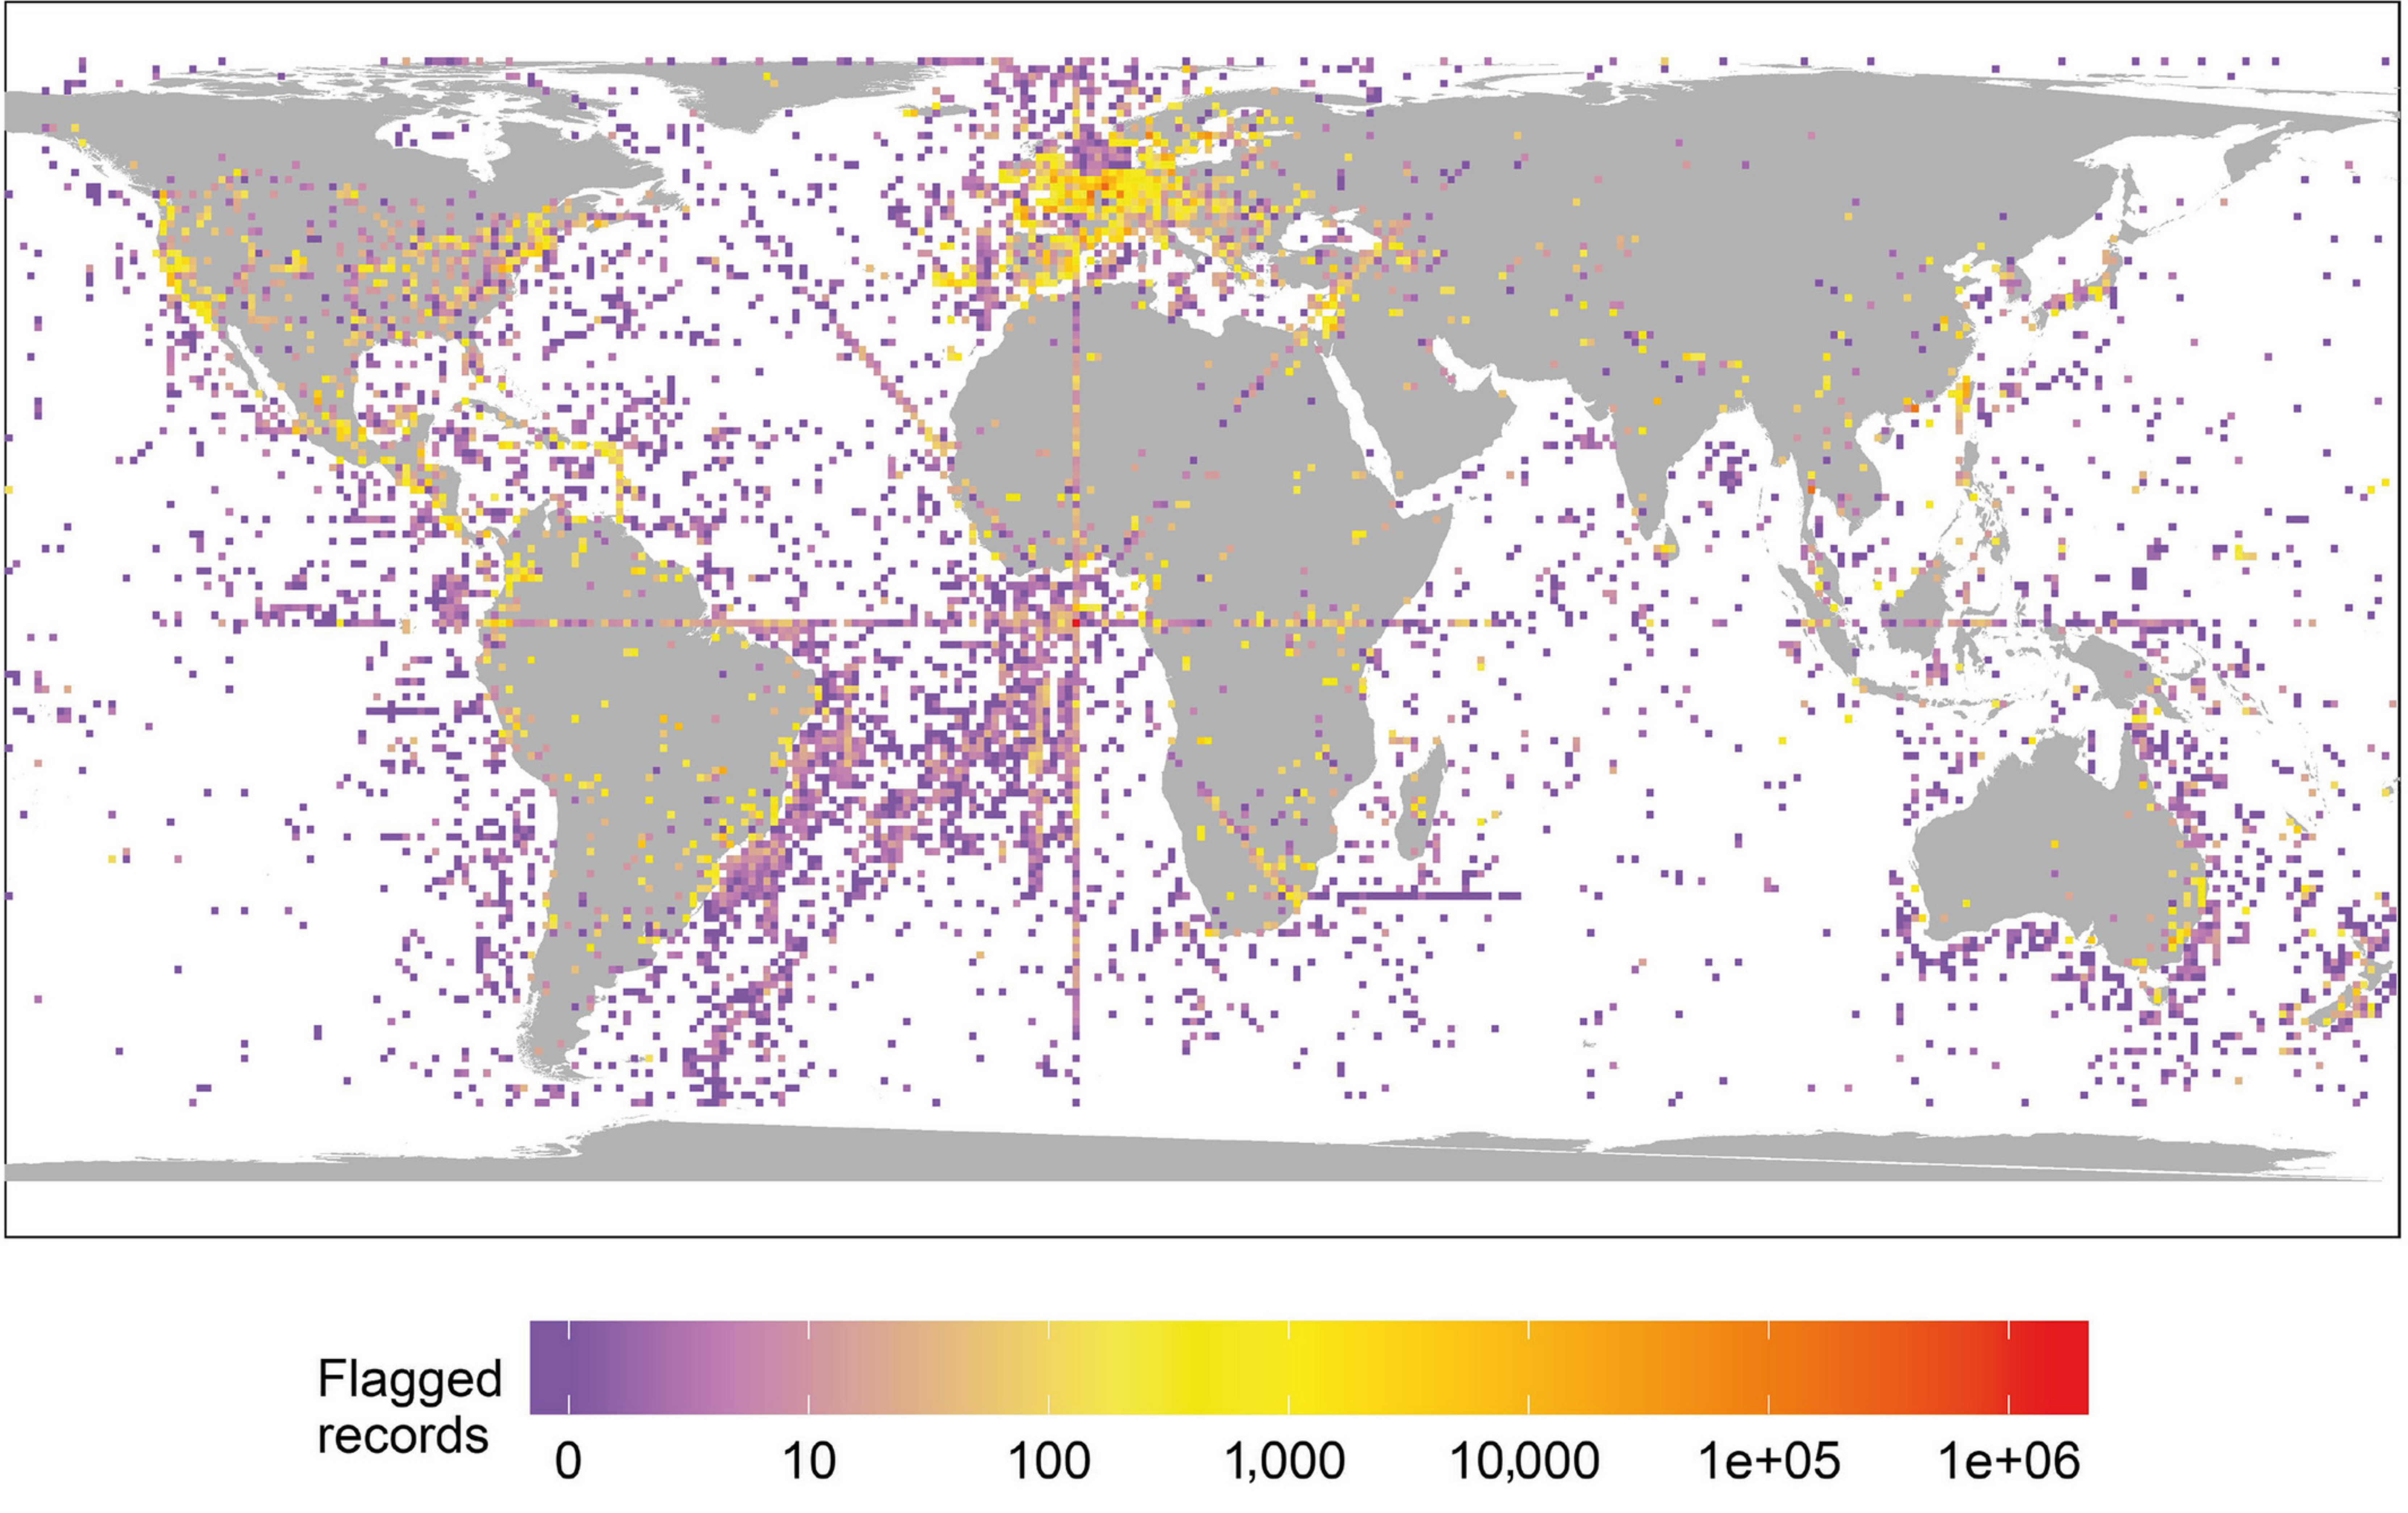
\includegraphics[width=5.9375in,height=4.16667in]{img/occ_bias.png}

\href{https://doi.org/10.1111/2041-210X.13152}{Zizka et al.~(2019)}
\end{frame}

\begin{frame}{Species occurrences}
\phantomsection\label{species-occurrences-8}
\textbf{sampbias}

\begin{itemize}
\tightlist
\item
  Statistical method to evaluate and visualize \textbf{geographic
  sampling biases}
\item
  Bias:
\end{itemize}

\begin{itemize}
\tightlist
\item
  Cities
\item
  Airports
\item
  Roads
\item
  Rivers
\end{itemize}

\includegraphics[width=3.64583in,height=4.16667in]{img/occ_bias_map1.jpg}
\includegraphics[width=4.16667in,height=4.6875in]{img/occ_bias_map.jpg}

\href{https://doi.org/10.1111/ecog.05102}{Zizka et al.~(2020)}
\end{frame}

\begin{frame}{Spatial analysis}
\phantomsection\label{spatial-analysis}
\textbf{Spatial units - Grids}
\end{frame}

\begin{frame}{Spatial analysis}
\phantomsection\label{spatial-analysis-1}
\textbf{Spatial units - Hexagons}
\end{frame}

\begin{frame}{Spatial analysis}
\phantomsection\label{spatial-analysis-2}
\textbf{Convex hull}
\end{frame}

\begin{frame}{Spatial analysis}
\phantomsection\label{spatial-analysis-3}
\textbf{Point density (kernel maps)}
\end{frame}

\begin{frame}{Spatial analysis}
\phantomsection\label{spatial-analysis-4}
\textbf{Species Distribution Modeling (SDMs)}

\href{https://www.cambridge.org/br/academic/subjects/life-sciences/ecology-and-conservation/habitat-suitability-and-distribution-models-applications-r}{Guisan
et al.~(2017)}
\end{frame}

\begin{frame}{Spatial analysis}
\phantomsection\label{spatial-analysis-5}
\textbf{Species Distribution Modeling (SDMs)}

\begin{itemize}
\tightlist
\item
  Generalized Linear Models (GLM) - binomial
\end{itemize}

\href{https://linkinghub.elsevier.com/retrieve/pii/S0304380002002041}{Guisan
et al.~(2002)}
\end{frame}

\begin{frame}{Spatial analysis}
\phantomsection\label{spatial-analysis-6}
\textbf{Species Distribution Modeling (SDMs)}

\begin{itemize}
\tightlist
\item
  \href{https://cran.r-project.org/web/packages/dismo/}{dismo}
\item
  \href{https://cran.r-project.org/web/packages/biomod2/}{biomod2}
\item
  \href{https://cran.r-project.org/web/packages/sdm/}{sdm}
\item
  \href{https://github.com/andrefaa/ENMTML}{ENMTML}
\item
  \href{https://model-r.github.io/modleR/}{modelR}
\item
  \href{https://cran.r-project.org/web/packages/ENMeval/}{ENMeval}
\item
  \href{https://sjevelazco.github.io/flexsdm/index.html}{flexsdm}
\item
  \href{https://cran.r-project.org/web/packages/SDMtune/}{SDMtune}
\item
  \href{https://cran.r-project.org/web/packages/wallace/}{wallace}
\item
  \href{https://cran.r-project.org/web/packages/ssdm/}{ssdm}
\item
  \href{https://gitlab.com/IanOndo/shinybiomod}{ShinyBIOMOD}
\end{itemize}

\includegraphics[width=4.375in,height=5.72917in]{img/sdm_sdm_pkg.png}

\href{https://github.com/helixcn/sdm_r_packages}{R packages}
\end{frame}

\begin{frame}{Landscape ecology}
\phantomsection\label{landscape-ecology}
\textbf{Habitat/non-habitat}
\end{frame}

\begin{frame}{Landscape ecology}
\phantomsection\label{landscape-ecology-1}
\textbf{Landscape metrics}
\end{frame}

\begin{frame}{Application: SN Platform}
\phantomsection\label{application-sn-platform}
\end{frame}

\section{Material}\label{material}

\begin{frame}{Articles}
\phantomsection\label{articles}
\begin{itemize}
\item
  \href{https://doi.org/10.1590/S2175-78602012000300017}{Giannini, T. C.
  et al.~(2012). Desafios atuais da modelagem preditiva de distribuição
  de espécies. Rodriguésia, 63(3), 733--749.}
\item
  \href{https://doi.org/10.1126/sciadv.aat4858}{Araújo, M. B. et
  al.~(2019). Standards for distribution models in biodiversity
  assessments. Science Advances, 5(1), eaat4858.}
\item
  \href{https://doi.org/10.1111/ecog.04960}{Zurell, D. et al.~(2020). A
  standard protocol for reporting species distribution models.
  Ecography, 43(9), 1261--1277.}
\item
  \href{https://doi.org/10.1080/13658816.2020.1798968}{Sillero, N., \&
  Barbosa, A. M. (2021). Common mistakes in ecological niche models.
  International Journal of Geographical Information Science, 35(2),
  213--226.}
\item
  \href{https://doi.org/10.1016/j.ecolmodel.2021.109671}{Sillero, N. et
  al.~(2021). Want to model a species niche? A step-by-step guideline on
  correlative ecological niche modelling. Ecological Modelling, 456,
  109671.}
\end{itemize}
\end{frame}

\begin{frame}{Books}
\phantomsection\label{books}
\begin{itemize}
\item
  \href{https://doi.org/10.1017/CBO9780511810602}{Franklin, J., \&
  Miller, J. A. (2009). Mapping species distributions: Spatial inference
  and prediction. Cambridge University Press.}
\item
  \href{https://press.princeton.edu/books/paperback/9780691136882/ecological-niches-and-geographic-distributions-mpb-49}{Peterson,
  A. T. (Org.). (2011). Ecological niches and geographic distributions.
  Princeton University Press.}
\item
  \href{https://jhupbooks.press.jhu.edu/title/mapping-disease-transmission-risk}{Peterson,
  A. T. (2014). Mapping disease transmission risk: Enriching models
  using biogeography and ecology. Johns Hopkins University Press.}
\item
  \href{https://doi.org/10.1017/9781139028271}{Guisan, A., Thuiller, W.,
  \& Zimmermann, N. E. (2017). Habitat Suitability and Distribution
  Models: With Applications in R. Cambridge University Press.}
\item
  \href{https://doi.org/10.1007/978-3-030-01989-1}{Fletcher, R., \&
  Fortin, M.-J. (2018). Spatial Ecology and Conservation Modeling:
  Applications with R. Springer International Publishing.}
\end{itemize}
\end{frame}

\begin{frame}{Muito obrigado!}
\phantomsection\label{muito-obrigado}
\begin{columns}[T]
\begin{column}{0.5\textwidth}
Acknowledgements:

\begin{itemize}
\tightlist
\item
  Mathias Pires
\item
  Miltinho
\item
  FlaPinto
\item
  Matheus Lima-Ribeiro
\item
  João Giovanelli
\end{itemize}
\end{column}

\begin{column}{0.5\textwidth}
Contact:

\href{mailto:mauricio.vancine@gmail.com}{\nolinkurl{mauricio.vancine@gmail.com}}
\href{https://mauriciovancine.github.io}{mauriciovancine.github.io}
\end{column}
\end{columns}

Slides por \href{https://mauriciovancine.github.io/}{Maurício Vancine},
feitos com \href{https://quarto.org/}{Quarto}. Código disponível no
\href{https://github.com/mauriciovancine/workshop-intro-r/blob/master/01_slides/slides.qmd}{GitHub}.
\end{frame}



\end{document}
